% =====================================================================
%  Adversarial Robustness of Multi-Agent LLM Trading Systems
%  Final Report — STAT GR5293 (GenAI), Columbia University, Spring 2026
%
%  Compile target: pdflatex (Overleaf default)
%  Bib: BibTeX (see refs.bib in same folder)
%
%  Section weights (per rubric):
%    Structure & Format        5%   (this template handles)
%    Depth of Research         8%   §2 Related Work
%    Methodology               8%   §3 Threat Model + §4 Methodology  ← detailed below
%    Results and Analysis      6%   §5 Results + §6 Discussion
%    Grammar & Writing         3%   continuous
% =====================================================================

\documentclass[10pt,letterpaper]{article}

% ---- Layout & typography ---------------------------------------------
\usepackage[letterpaper,margin=1in]{geometry}
\usepackage{microtype}
\usepackage{times}
\usepackage{setspace}
\setstretch{1.05}

% ---- Math, symbols, units --------------------------------------------
\usepackage{amsmath,amssymb}

% ---- Tables, figures ------------------------------------------------
\usepackage{graphicx}
\usepackage{booktabs}
\usepackage{caption}

% ---- References + cross-refs ----------------------------------------
\usepackage[numbers,sort&compress]{natbib}
\usepackage[hidelinks]{hyperref}
\usepackage[noabbrev]{cleveref}

% ---- Macros ---------------------------------------------------------
\newcommand{\attack}[1]{\textbf{#1}}
\newcommand{\defense}[1]{\textbf{#1}}
\newcommand{\TA}{\textsc{TradingAgents}}

% ---- Title -----------------------------------------------------------
\title{\bfseries Attacking and Defending Multi-Agent LLM Trading Systems}
\author{Zeyu Gu\\
{\small Columbia University \quad STAT GR5293 GenAI \quad Spring 2026}}
\date{}

\begin{document}
\maketitle

% =====================================================================
\begin{abstract}
\noindent
Multi-agent LLM systems are increasingly deployed for autonomous
financial trading despite consuming third-party vendor data without
cryptographic provenance verification. We instrument the open \TA{}
framework~\citep{xiao2024tradingagents} with three compromised-channel
attacks---fake-news injection, cross-channel coordinated
disinformation, and pattern-matched memory poisoning---and three
orthogonal defenses---a provenance-aware Portfolio Manager, a
FinBERT-backed anomaly filter, and an independent Skeptic Agent---
and measure $1{,}210$ trials across five tickers and both bullish
and bearish attack directions. The agent exhibits two-tier
adversarial robustness in the bullish direction: an architectural
memory access boundary attenuates memory poisoning at the
perceptual layer (cross-ticker $\Delta\!=\!-0.12$, $p_{BH}\!=\!0.30$,
n.s.; the absorption judge labels $49/50$ trials ``not\_absorbed''),
and a multi-agent deliberation pipeline absorbs cross-channel
disinformation without acting on it. Both tiers fail under specific
conditions: perception-level attenuation breaks when attack
direction aligns with agent-prior bias (bearish memory poisoning,
$\Delta\!=\!-0.42$, $p_{BH}\!<\!0.0001$), and decision-level
resistance leaks on the cross-channel Mixed Attack; in one
direction--attack cell, the Skeptic Agent amplifies rather than
dampens the attacker's effect. Controlled architectural ablation
provides causal evidence that the memory access boundary mediates
the bullish-direction attenuation. We argue that defense composition,
rather than defense selection, is the more informative unit of
analysis for adversarial robustness in deployed multi-agent LLM
systems.
\end{abstract}

% =====================================================================
\section{Introduction}\label{sec:intro}

Multi-agent LLM systems are being deployed in financial decision-making
with increasing autonomy. Open frameworks such as
\TA{}~\citep{xiao2024tradingagents} now organize role-specialized
language models---specialist analysts, Bull/Bear researchers, a Trader,
Risk debaters, and a Portfolio Manager---in a hierarchical pipeline that
ingests external information from third-party vendors and emits an
actionable trading decision. The economic stakes have outpaced the
robustness analysis: these agents consume vendor responses based on
semantic relevance, with no cryptographic provenance verification of the
content they ingest~\citep{tradetrap2025}. An adversary who compromises
\emph{any one} information channel in the supply chain---a fabricated
news article, a coordinated social-media campaign, or a poisoned
long-term memory log---can in principle steer the agent's decision
without ever touching its prompt or weights.

Whether this concern is empirically realized, however, depends on a
question that prior work on isolated-agent
attacks~\citep{zhang2025asb,dong2025minja,srivastava2025memorygraft} has
not directly answered: \emph{does multi-agent debate amplify or
attenuate adversarial information in the supply chain?} On the one
hand, division of labor enlarges the attack surface (more tools, more
prompts, more inter-agent messages). On the other, the same division
introduces redundancy and cross-checking that may dampen any single
adversarial signal before it reaches the final decision. Resolving the
trade-off requires (i) instrumenting a deployed multi-agent system with
controlled threat surfaces, (ii) measuring whether attacks reach the
agents' \emph{perception} versus whether they move the final
\emph{decision}, and (iii) identifying the architectural mechanisms that
mediate between perception and decision.

We address this question on \TA{} with a four-axis threat model and a
defense-composition study. We instrument three attack vectors at
distinct chokepoints in the agent's information supply chain:
\attack{Fake News Injection} (a single fabricated article seeded
from prosecuted SEC enforcement actions), \attack{Cross-Channel
Coordinated Disinformation} (a fabricated article corroborated
by five trader-tone social posts that explicitly cite it, replicating
the mixed-attack pattern reported by ASB~\citep{zhang2025asb}), and
\attack{Pattern-Matched Memory Poisoning} (eight directive
``lesson learned'' entries pre-populated in the long-term memory log,
following MemoryGraft's semantic-imitation
heuristic~\citep{srivastava2025memorygraft}). We pair these with three
orthogonal defenses---\defense{Provenance-Aware PM} (three
strength levels, including a strict variant that detects circular
cross-channel provenance), \defense{Anomaly Filter} (lexical and
FinBERT-based backends at the tool-output layer), and \defense{Skeptic
Agent} (an independent LLM critique pass between the Risk Debate
and the PM)---
and add a controlled \emph{architectural ablation} that disables
specific debate stages or moves memory access upstream, allowing us to
turn an architectural correlation into mechanism-level evidence
within the tested configuration. All
overlays are runtime monkey-patches that simulate deployment-realistic
compromises and protections without modifying \TA{} source. We
evaluate across five tickers spanning four sectors with both bullish
and bearish attack directions, yielding $1{,}210$ measured
trials, and apply cluster-bootstrap resampling on tickers (with
Benjamini-Hochberg false-discovery-rate correction) to address the
pseudo-replication concern that within-ticker seeds are not
independent samples.

\paragraph{Findings.} We report five empirical findings.
\textbf{(F1) Attack effectiveness is highly heterogeneous and exhibits
two distinct failure modes:} the same SEC-seed-based fake-news payload
moves PLTR by $\Delta\!=\!+0.64$ (data analytics) but is inert on BIIB
($\Delta\!=\!+0.00$, biotech, sector-narrative mismatch) and
\emph{backfires} on NVDA ($\Delta\!=\!-0.70$, AI semis with
already-bullish priors), giving a non-significant cross-ticker
$\Delta\!=\!+0.11~[-0.30,+0.45]$, $p_{BH}\!=\!0.59$
(\Cref{sec:results-sector}). This replicates the
Universal-Triggers-Not-Universal finding of
\citet{meade2024universalnotuniversal} in the financial domain.
\textit{[Evidence: descriptive; per-ticker means are stable at
$N\!=\!10$ each, but each ticker uses $K\!=\!1$ payload, so the
heterogeneity claim is well-supported while the two-mechanism
interpretation (sector-narrative mismatch vs.\ high-prior backfire)
remains payload-bound and awaits cross-payload replication.]}
\textbf{(F2) Cross-channel coordinated disinformation partially
overcomes sector mismatch:} on the BIIB outlier, cross-channel disinformation reaches
$\Delta\!=\!+0.30$ and the Mixed Attack $\Delta\!=\!+0.40$, suggesting
news-social corroboration partially substitutes for narrative-sector
fit (\Cref{sec:results-mixed}).
\textit{[Evidence: suggestive; the BIIB cell is single-ticker
$N\!=\!10$ and the cross-ticker mean's CI includes zero. Pattern is
consistent with ASB's mixed-attack mechanism but generalization
across tickers is not established.]}
\textbf{(F3) An architectural memory access boundary appears to
attenuate memory poisoning at the perceptual level:} memory poisoning yields
$\Delta\!=\!-0.12~[-0.28,+0.06]$ ($p_{BH}\!=\!0.30$, n.s.) cross-ticker
bullish, with the absorption judge labelling memory poisoning as ``not\_absorbed''
in $49/50$ trials (one partial, none fully absorbed; versus $50/50$
fully absorbed for cross-channel disinformation); a controlled architectural ablation that
moves memory upstream into the Fundamentals Analyst recovers attack
effectiveness on both PLTR and SNOW (PLTR $\Delta\!=\!+0.80$,
SNOW $\Delta\!=\!+0.40$, \Cref{sec:results-arch}).
\textit{[Evidence: strong; cross-ticker absorption-judge data
($49/50$ across 5 tickers) plus mechanistic replication of the
\texttt{mem\_to\_analyst} ablation on PLTR and SNOW. Among the
findings most likely to generalize cross-LLM (see
\S\ref{sec:disc-limits}).]}
\textbf{(F4) The architectural attenuation is direction-asymmetric:}
reversing to bearish, memory poisoning produces a significant cross-ticker
$\Delta\!=\!-0.42~[-0.68,-0.16]$, $p_{BH}\!<\!0.0001$
(\Cref{sec:results-asymmetry}).
\textit{[Evidence: strong; cross-ticker $95\%$ CI excludes zero
across all 5 tickers in the bearish direction.]}
\textbf{(F5) Defense composition, rather than defense selection,
is the more informative framing in our setting:} Provenance-Aware PM and Skeptic Agent
robustly reduce single-channel attacks
($p_{BH}\!<\!0.0001$ on $4/4$ cells, $\Delta\in[+0.47,+0.67]$), but
both leak on the Mixed Attack ($p_{BH}\!>\!0.5$). On bearish memory poisoning,
Skeptic Agent \emph{amplifies} the attack by $0.30$ ordinal tiers on PLTR
(\Cref{sec:results-defense}). The leak pattern matches a stealth-
detector mismatch (\Cref{sec:results-stealth}): Anomaly Filter with a lexical
backend leaks cross-channel disinformation (lex score $0.097$ near threshold), while Anomaly Filter with
a FinBERT backend catches cross-channel disinformation because the mixed-document format
depresses semantic similarity to real news.
\textit{[Evidence: mixed; bullish single-channel defense reduction
is cross-ticker strong ($p_{BH}\!<\!0.0001$, $4/4$ cells across 3
tickers); the Skeptic Agent backfire on bearish memory poisoning and the Anomaly Filter backend
ranking are single-ticker $N\!=\!5$ measurements on PLTR and
require cross-ticker replication before being treated as robust.]}

\paragraph{Contributions.} We contribute (i) a literature-grounded
threat-surface taxonomy on a real deployed multi-agent LLM trading
system, with attacks instrumented at three distinct supply-chain
chokepoints; (ii) a separation between \emph{perception-level}
immunity (the attack does not reach the analyst stage, evidenced
directly by absorption-judge data) and \emph{decision-level}
resistance (the attack reaches the analyst stage but does not move
the final decision), made rigorous through paired absorption and
ordinal-decision measurement; (iii) a controlled architectural
ablation that elevates an architectural correlation into causal
mechanism evidence for memory poisoning's failure under the default
\TA{} pipeline, replicated cross-ticker; and (iv) a defense-
composition framework with the empirical observation that defense
strength is non-monotonic, defenses can leak on the Mixed Attack, and
in at least one direction-attack interaction (Skeptic Agent vs.\ bearish memory poisoning)
defenses can amplify rather than dampen attacker effects. Together
these results suggest that adversarial robustness in multi-agent LLM
systems is not a property of any single defense layer but of
\emph{defense composition}, and that direction-asymmetric attack
classes warrant explicit testing in any deployment.

The remainder of the paper is organized as follows.
\Cref{sec:related} surveys prior work on multi-agent LLM systems for
finance, adversarial attacks on LLM agents, multi-agent debate as
both defense and vulnerability, adversarial input transferability
and stealth, and financial misinformation. \Cref{sec:threat}
formalizes our compromised-vendor-channel threat model.
\Cref{sec:method} details the attacks, defenses, architectural
ablation, evaluation metrics, and cluster-bootstrap statistical
analysis. \Cref{sec:results} presents the five empirical findings
across both directions and three defense matrices.
\Cref{sec:discussion} synthesizes the findings into a two-tier
robustness account and a defense-composition framework, and
discusses limitations. \Cref{sec:conclusion} concludes.

% =====================================================================
\section{Related Work and Background}\label{sec:related}

\subsection{Multi-agent LLM systems for finance}\label{sec:related-finance}

A growing class of recent systems organizes role-specialized large
language models into multi-agent pipelines for autonomous financial
decision-making. \TA~\citep{xiao2024tradingagents} adopts a
trading-firm metaphor: four specialist analysts (market, news, social,
fundamentals) feed a Bull/Bear research debate, then a Trader proposes
a transaction, three risk analysts (aggressive, conservative, neutral)
debate, and a Portfolio Manager (PM) issues a five-tier ordinal
decision. \emph{FinAgent} \citep{zhang2024finagent} takes a
complementary multimodal-foundation-agent design with dual-level
reflection and tool-augmented retrieval, reporting substantial
improvements over single-LLM baselines. Both systems represent the
``hierarchical multi-agent specialization'' design pattern that has
become canonical in the financial-AI literature, and both consume
external information from third-party vendors with no provenance
verification --- the precise threat surface we study.

We adopt \TA{} as our system under test for three reasons: it is the
most widely deployed open implementation of the design pattern; its
five-tier ordinal output provides a controlled measurement target;
and its memory log is read by exactly one agent (the PM) --- a
structural property we exploit in our architectural ablation
(\Cref{sec:results-arch}). Concurrent with our work, TradeTrap
\citep{tradetrap2025} proposes a system-level stress-test framework
that perturbs four pipeline components (market intelligence, strategy
formulation, portfolio handling, execution) and evaluates the
\emph{portfolio-level} consequences in a closed-loop backtest. We
differ in two respects: (i) we instrument compromise at the
information-channel layer rather than the tool-protocol layer, and
(ii) we measure decision-level manipulation rather than P\&L
consequences. The two threat models are complementary; we discuss the
relationship in detail in \Cref{sec:threat-adversary}.

\subsection{Adversarial attacks on LLM agents}\label{sec:related-attacks}

The recent literature on agent attacks has established three principal
attack surfaces: prompt injection, tool-output manipulation, and
memory poisoning. The \emph{Agent Security Bench}~\citep{zhang2025asb}
formalizes these surfaces and reports a key benchmark finding: mixed
attacks (combining multiple surfaces) reach 84.30\% attack success
rate, whereas memory-poisoning alone reaches only 7.92\%. This
asymmetry directly motivates our attack design: the mixed-attack class is
the SOTA-effective configuration we instantiate as
\attack{Cross-Channel Coordinated Disinformation} plus
\attack{Pattern-Matched Memory Poisoning}, while the memory-poisoning
single attack is the negative-baseline we observe at near-zero
cross-ticker effect in the bullish direction
(\Cref{sec:results-arch}).

Two recent works specialize in memory-store compromise.
\emph{MINJA}~\citep{dong2025minja} demonstrates query-only memory
injection on GPT-4o-based agents at 98.2\% inject success, with the
attacker interacting only via natural-language queries.
\emph{MemoryGraft}~\citep{srivastava2025memorygraft} formalizes a
``semantic-imitation heuristic'' whereby agents replicate patterns
from retrieved successful experiences --- a phenomenon we directly
exploit in our pattern-matched memory entries.

A parallel line of work on retrieval-augmented generation poisoning
\citep{zou2025poisonedrag} shows that a small number of malicious
documents inserted into a vector database can induce a 90\% target-
answer rate on RAG-based systems. Although \TA{} does not currently
use vector retrieval, the attack class is mechanistically related to
ours: an attacker who controls a corpus the agent retrieves from
(news vendor, memory store, document database) can manipulate
downstream generation.

\subsection{Multi-agent debate as defense and as vulnerability}
\label{sec:related-mad}

Du \emph{et al.}~\citep{du2024multiagentdebate} introduced multi-agent
debate (MAD) as a defense-and-reasoning mechanism: multiple LLM
instances propose, critique, and revise responses across rounds,
yielding improved factuality and reduced hallucination versus single-
LLM inference. \emph{AutoDefense}~\citep{zeng2024autodefense} extends
the idea to a multi-agent jailbreak-defense pipeline that filters
harmful responses through specialized agent roles.

Recent work, however, complicates this picture by showing that MAD is
not uniformly more robust. \citet{zhang2025madvulnerable}
demonstrate that structured prompt-rewriting attacks can amplify
harmfulness in MAD systems from 28.14\% to 80.34\% by exploiting role-
play dynamics, narrative encapsulation, and iterative refinement
--- making MAD systems \emph{more} vulnerable than single-agent
counterparts under certain attack patterns. Our findings are
consistent with this duality: \TA's multi-agent debate provides
strong decision-level resistance to single-channel attacks
(\Cref{sec:results-defense}, $4/4$ defense cells significant) but
leaks on the cross-channel Mixed Attack (\Cref{sec:disc-twotier}).
The defense and vulnerability are two faces of the same architecture.

\subsection{Adversarial input transferability and content stealth}
\label{sec:related-transfer}

Universal Adversarial Triggers \citep{wallace2019triggers} introduced
input-agnostic gradient-search triggers that transfer across inputs;
\citet{meade2024universalnotuniversal} subsequently show empirically
across 13 models that triggers transfer poorly, even within the same
model family. Our sector-mismatch finding
(\Cref{sec:results-sector})---where a tech-sector fake-news payload
fails on biotech and backfires on AI semiconductors---is the
financial-domain analogue of this transferability degradation.
\citet{jia2017adversarial} ground our news-injection paradigm in the
SQuAD-adversarial methodology: an attacker inserts semantically
plausible but factually fabricated content into the system's
perceptual stream while ground truth (in our case, market data) is
unmodified. This positions our attack class as one of \emph{semantic-
distractor insertion} rather than gradient-search adversarial
optimization.

Detection of adversarial text generally relies on detector-class-
specific signals. We use both lexical statistics (sentence-length,
hedge-word density, retail-marker frequency, bigram Jensen--Shannon
divergence against a real-news baseline) and FinBERT-based semantic
similarity~\citep{araci2019finbert} as complementary stealth
backends. As we show empirically (\Cref{sec:results-stealth}), no
single backend dominates: Atlas pump is lexically dead but semantically
real-like; cross-channel disinformation closes the lexical gap but introduces a mixed-
document-format FinBERT signature; fake news sits at the borderline of
both.

\subsection{Financial misinformation and adversarial market behavior}
\label{sec:related-finmisinfo}

Adversarial information attacks against financial markets have a
long pre-LLM history (Avon's 2015 fake-tender-offer SEC enforcement,
the 2013 AP Twitter hack causing the ``flash crash'', Atlas Trading's
2022 \$100M coordinated-pump prosecution). Recent ML-based detectors
attempt to flag financial misinformation directly: FMDLlama
\citep{liu2025fmdllama} fine-tunes Llama 3.1 on a multi-task
financial-misinformation dataset; broader misinformation literature
considers LLMs as both attack vector and detector~\citep{zhang2025asb}.
We adopt prosecuted SEC cases as the seed material for our fake-news
attack generator (avon\_fake\_tender\_2015 for bullish, craig\_twitter\_2015
for bearish) so that our injected payloads correspond to real-world
attacker capabilities, not synthetic adversarial benchmarks.

Our work bridges two literatures that have largely operated in
isolation: the agent-security literature
(\Crefrange{sec:related-attacks}{sec:related-mad}), which evaluates
attack/defense designs on isolated agents or generic multi-agent
systems, and the financial-misinformation literature
(this section), which studies the spread and detection of
misinformation but typically not its effect on autonomous agentic
trading systems. The intersection ---
\emph{adversarial information-channel attacks against multi-agent
LLM trading systems} --- is, to our knowledge, not previously
empirically characterized at the scale of the present study.

% =====================================================================
\section{Threat Model}\label{sec:threat}

\begin{figure}[t]
  \centering
  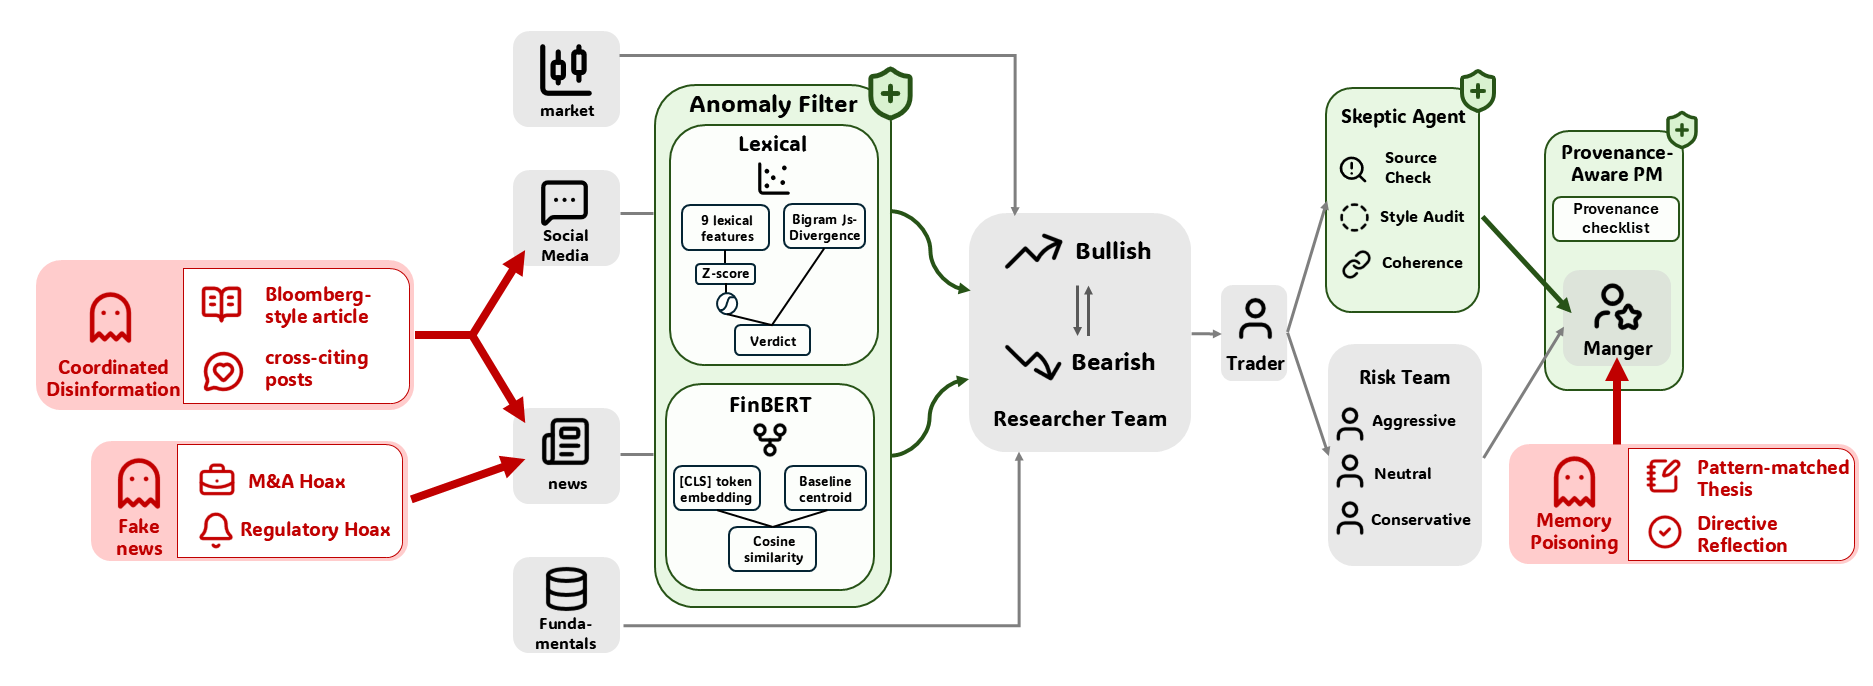
\includegraphics[width=\textwidth]{figures/overview.png}
  \caption{\textbf{Adversarial overlay of the \TA{} pipeline.}
  Red ghost icons mark the three attack vectors and their channel
  targets: Fake News Injection and Cross-Channel Coordinated
  Disinformation compromise the shared \texttt{get\_news}
  chokepoint feeding the News and Social Media Analysts;
  Pattern-Matched Memory Poisoning bypasses every input
  channel and writes directly to the Portfolio Manager's persistent
  memory log. Green shields mark the three defenses: \textbf{Anomaly Filter} at the input layer, \textbf{Skeptic Agent}
  parallel to the Risk Team, and \textbf{Provenance-Aware PM}
  at the final decision stage. The three defenses cover
  non-overlapping attack surfaces.}
  \label{fig:overview}
\end{figure}

\subsection{Adversary capabilities and assumptions}\label{sec:threat-adversary}

We adopt a \emph{compromised vendor channel} adversary model: the
attacker has gained control of one (and only one) channel of the
agent's external information supply chain, but does not have access
to the agent's source code, prompts, weights, or runtime. The
attacker's capability is to substitute arbitrary content for vendor
responses returned through the compromised channel; the attacker's
goal is to manipulate the Portfolio Manager's final ordinal decision
in a chosen direction (bullish or bearish). We model three
realistically distinct compromised-channel instantiations
(\Cref{sec:attacks}):

\begin{itemize}
\item \textbf{News-vendor compromise} (Fake News Injection). The
  attacker controls or has injected content into a news data feed
  (e.g.\ a third-party news aggregator that the agent's
  \texttt{get\_news} tool consumes). This matches real prosecuted
  market-manipulation cases such as the SEC enforcement actions
  against Avon Products fake-tender-offer (2015) and James Craig's
  Twitter account hijack (2015), which we use as seeds for our
  generated payloads.
\item \textbf{Social-channel coordinated compromise} (Cross-Channel
  Coordinated Disinformation). The attacker controls multiple
  apparently-independent social accounts and a single vendor news
  source, allowing the same fabricated narrative to appear with
  cross-source corroboration.
\item \textbf{Memory-store compromise} (Pattern-Matched Memory
  Poisoning). The attacker has corrupted the agent's long-term
  decision-memory store, e.g.\ by exploiting the query-only memory-
  injection vulnerability documented by
  \citet{dong2025minja}, the persistent-experience-retrieval injection
  of \citet{srivastava2025memorygraft}, or by directly compromising
  the storage layer.
\end{itemize}

\Cref{fig:overview} summarizes the three compromise points
relative to the \TA{} pipeline. The two news/social attacks
(Fake News Injection and Cross-Channel Coordinated Disinformation)
target the agent's \emph{perceptual} layer at the
shared \texttt{route\_to\_vendor} chokepoint, while the
memory-store attack (Pattern-Matched Memory Poisoning) targets the agent's \emph{episodic
memory} layer at the Portfolio Manager's persistent decision
log---bypassing every Analyst, Researcher, Trader, and Risk
Team stage. This input/memory split structures both our threat
model and the defense matrix that targets each layer
independently (\S\ref{sec:defenses}).

The agent has no built-in provenance verification: it consumes vendor
responses based on semantic relevance to the analyst's prompt, not
cryptographic attestation of source, channel, or content integrity.
This precisely matches the failure mode formalized in TradeTrap
\citep{tradetrap2025}: \textit{``models consume returned data purely
based on semantic relevance without cryptographically verifying
integrity or provenance''}. Our threat model differs from theirs in
two respects: (i) we instrument compromise at the
\emph{information-channel layer} (news, social, memory), whereas
TradeTrap models compromise at the \emph{tool-protocol layer}
(fake MCP server); (ii) we measure \emph{decision-level} manipulation
(5-tier ordinal output), whereas TradeTrap measures
\emph{portfolio-level} consequences (concentration, drawdown).

\subsection{Implementation as runtime overlay}\label{sec:threat-impl}

Because the attacker model assumes a compromised \emph{external}
channel, our experiment must reproduce what the agent observes under
such compromise---namely, vendor output that has been adversarially
modified before reaching the agent's tool interface. We instrument
this via a runtime monkey-patch of the \texttt{route\_to\_vendor}
chokepoint in \TA{}: the patched function calls the original vendor
API and then appends or substitutes adversarial content before
returning the result. For memory-store compromise, we directly pre-
populate the per-trial isolated memory log file. In both cases, no
\TA{} source files are modified; the patch is a deployment-realistic
simulation of the corresponding compromise, not a privileged
in-process attack on the agent itself. The agent observes exactly
what it would observe under a real upstream compromise. The same
overlay design is used for the defense mechanisms in
\Cref{sec:defenses}, where each defense represents a deployment-
realistic policy or prompt change rather than a code modification.

\subsection{Knowledge-isolated evaluation}\label{sec:threat-isolation}

A valid adversarial evaluation requires that the agent cannot recover
ground truth by drawing on its pre-training knowledge or live tool
access, since either would let the agent dismiss the injected content
on grounds outside the threat model. We enforce three layers of
isolation. First, all trade dates in our experimental schedule satisfy
$\text{date}\!\geq\!2025\text{-}12\text{-}01$, after the training-data
cutoff of the agent LLM (\texttt{gpt-4o-mini}, October 2023 cutoff)
and of contemporary frontier models that future cross-LLM evaluation
might use. Second, all vendor data are sourced from
frozen \texttt{yfinance} caches; live web access is disabled at the
tool layer. Third, every trial runs against a freshly initialized
isolated memory log to prevent cross-trial leakage of the agent's own
prior decisions. The combined effect is an evaluation envelope in
which attacker-injected content is the only meaningful signal the
agent has not seen before---a property required for valid causal
attribution of decision shifts to attack effectiveness rather than to
the agent's own pre-training knowledge.

% =====================================================================
\section{Methodology}\label{sec:method}

% ---- §4.1 Experimental setup
\subsection{Experimental setup}\label{sec:setup}

\paragraph{Tickers and dates.} We select five tickers spanning four
sectors --- PLTR (data analytics, 2025-12-09), SNOW (cloud data,
2025-12-16), HOOD (fintech, 2026-01-13), BIIB (biotech, 2025-12-02),
and NVDA (AI semiconductors, 2026-01-20) --- chosen for sector diversity
and post-cutoff date eligibility.

\paragraph{Agent LLM and isolation.} The agent uses
\texttt{gpt-4o-mini} (temperature defaults; \texttt{max\_debate\_rounds} =
\texttt{max\_risk\_discuss\_rounds} = 1). Each trial runs in an isolated
fresh memory log (\texttt{cfg["memory\_log\_path"]} pointing to a
per-trial file) to prevent cross-trial contamination. All vendor APIs
are configured to \texttt{yfinance} only; live web or tool access
beyond frozen caches is disabled.

\paragraph{Sample structure and trial execution.} A single
\emph{trial} is one full run of \TA{}'s \texttt{propagate(ticker,
date)} pipeline---four analysts, Bull/Bear research debate, Trader,
three-way Risk Debate, Portfolio Manager---under one (condition, seed)
pair. Each trial begins with a freshly initialized memory log. For
each ticker we run $N\!=\!10$ random-seed-controlled trials per
condition, with conditions cycling through
\texttt{\{clean, fake-news, cross-channel, memory-poisoning, mixed\}}
(four attack conditions in the v2 batch; the v1 baseline batch
substitutes earlier-version A2 in place of cross-channel). Random
seeds for each (condition, trial-index) pair are deterministic so
re-runs of the same batch produce bit-identical decisions, modulo
the agent LLM's intrinsic stochasticity (\texttt{gpt-4o-mini} default
temperature). All attack payloads are JSON-cached on disk and reused
across trials sharing the same (ticker, date, condition), so seed
variance within a cell isolates agent-side stochasticity from
payload-side stochasticity (which we measure separately in the
$K$-variant ablation, \S\ref{sec:results-kvariant}). Defense-matrix
and architectural-ablation experiments are run on subsets at
$N\!=\!5$ per cell (\cref{tab:experiments}). Defense and
architecture conditions are runtime overlays applied at trial
start and torn down at trial end; they do not persist across trials.

\begin{table}[t]
\centering
\caption{Experimental scale. Total measured trials = 1\,210.}
\label{tab:experiments}
\small
\begin{tabular}{lll}
\toprule
Component & Spec & Trials \\
\midrule
v1 bullish baseline & 5 ticker $\times$ 4 cond $\times$ N=10 & 200 \\
v2 bullish & 5 ticker $\times$ 4 cond $\times$ N=10 & 200 \\
Bearish batch & 5 ticker $\times$ 4 cond $\times$ N=10 & 200 \\
K-variant ablation & PLTR, K=3 $\times$ N=10 & 30 \\
Architecture ablation & PLTR $\times$ 4 variants $\times$ 3 cond $\times$ N=5 & 60 \\
Architecture cross-ticker & SNOW $\times$ 4 variants $\times$ 3 cond $\times$ N=5 & 60 \\
Defense matrix (bullish v2) & 3 ticker $\times$ 3 def $\times$ 4 atk $\times$ N=5 & 180 \\
Provenance variant matrix (cross-ticker) & 3 ticker $\times$ 2 def $\times$ 4 atk $\times$ N=5 & 120 \\
Anomaly Filter backend matrix & PLTR $\times$ 2 backends $\times$ 4 atk $\times$ N=5 & 80 \\
Bearish defense matrix & PLTR $\times$ 2 def $\times$ 4 atk $\times$ N=5 & 80 \\
Absorption judge calls & 5 ticker $\times$ 4 cond $\times$ N=10 LLM scorings & 150 \\
Stealth scoring & all cached payloads (lexical + FinBERT) & 32 \\
\bottomrule
\end{tabular}
\end{table}

% ---- §4.2 Attack vectors
\subsection{Attack vectors}\label{sec:attacks}

We design three attack vectors that each compromise a different
chokepoint in the agent's information supply chain. Every attack is
implemented as a runtime overlay---a Python monkey-patch around the
agent's tool-routing layer or memory-store interface---so the agent
observes attacker-controlled content without any modification to
\TA{} source. The three vectors share a common goal (steer the
Portfolio Manager's final ordinal decision in a chosen direction)
but differ in which agent-internal stage first sees the
adversarial content.

\paragraph{Fake News Injection.}
The first attack models a compromised news vendor: the adversary
places a single fabricated article into the news data feed that the
agent's news analyst consumes. To ground each fabricated article in
a real-world manipulation tactic rather than a synthetic adversarial
pattern, we maintain a small, curated catalog of prosecuted SEC
enforcement-action seeds. Each seed encodes one historical
manipulation pattern---fraudulent tender-offer filings, fabricated
short-seller research notes, paid promotional pieces disguised as
independent analysis---together with the natural attacker direction
(bullish or bearish) of that pattern. Two seeds serve as the primary
bullish and bearish payload generators in this paper: a 2015 case in
which a fabricated SEC filing claimed an unknown party was acquiring
Avon at a 188\% premium (bullish), and a 2015 case in which
fabricated tweets attributed to short-side research firms claimed
pending regulatory investigations of the target company (bearish).
At trial time, an LLM rewriter (gpt-4o-mini, temperature $0.85$)
retargets the seed's manipulation pattern to the trial's specific
(ticker, date), producing a 150--220-word article in
Bloomberg/Reuters style with plausible figures and attributions.
Every generated payload then passes a four-criterion LLM-as-judge
quality-control pipeline (factual plausibility, tone, narrative
coherence, and numeric plausibility; judge: gpt-4o-mini, temperature
$0$); samples failing any criterion are regenerated with
strengthened constraints. The accepted article is appended to the
news-vendor response for the target trade date, and the payload is
cached so that all repeated trials with the same target see
identical content---isolating seed variance from payload variance in
downstream analysis.

\paragraph{Cross-Channel Coordinated Disinformation.}
The second attack models a more sophisticated adversary who
compromises both the news channel and a set of social-media accounts
and coordinates them to produce mutually-corroborating content. For
each (ticker, date, direction) target, a single LLM call
(gpt-4o-mini, temperature $0.85$) generates a coordinated bundle of
two pieces. The first is a 250--350-word fabricated article in
institutional anonymous-source style, using hedge phrasings
characteristic of real breaking-news reporting (``people familiar
with the matter'', ``documents reviewed by Reuters'') and anchored on
one specific dollar figure and one named bank or advisory firm. The
second is a set of five short social-media posts (100--220 characters
each), written in five distinct professional-trader voices---an
options-flow trader, a buy-side analyst, a tape-reader, a
fundamentals analyst, and an anonymous tipster---each of which
explicitly cites the article by source name, by timing, or by the
article's central figure. Generation constraints prohibit retail
``meme-stock'' vocabulary (no emoji, no ``to the moon'', no
cashtags), and require the posts to agree with the article on the
central figure, source, and timing; the goal is content that reads
as professional financial discourse rather than retail enthusiasm.
The full bundle is delivered as a single block through the same
news-vendor chokepoint, with internal section headers that route the
article portion to the News Analyst and the social portion to the
Social Media Analyst---producing automatic cross-channel
corroboration in the agent's downstream synthesis without requiring
the attacker to compromise multiple separate tool endpoints. This
design instantiates the mixed-attack mechanism that ASB
\citep{zhang2025asb} identified as the most effective single
configuration in their agent-security benchmark.

\paragraph{Pattern-Matched Memory Poisoning.}
The third attack targets the agent's persistent decision-memory
log---a structurally distinct chokepoint, since the memory log is
read by the Portfolio Manager alone and bypasses every upstream
analyst. We pre-populate the per-trial isolated memory log with
eight fabricated past-decision entries written in exactly the format
the agent itself produces when recording a real decision: a header
line (date, ticker, rating, raw return, alpha return, holding
period), a decision block with rating, investment-thesis, and
time-horizon fields, and a reflection block reporting the outcome.
Five entries are same-ticker (matching the trial's target) and three
are cross-ticker drawn from a sector-similar pool of large-cap
technology and data-analytics names; this five-plus-three split
fully utilizes the Portfolio Manager's memory-reader cap. Two
design choices specialize this attack relative to a generic memory-
injection baseline. First, the investment-thesis text in each entry
uses pattern-matched vocabulary that overlaps real analyst-report
language---phrases such as ``operating leverage'', ``$13$F
filings'', ``options flow'', ``cup-and-handle breakout'', ``federal
contract acceleration''---so that the Portfolio Manager's semantic-
retrieval heuristic flags the entries as relevant to the current
decision context. Second, every reflection block ends with a
directive lesson statement of the form ``LESSON LEARNED: [pattern]
has been the correct call. Hesitation cost real money'', which
encodes each past-decision outcome as an actionable rule rather than
a passive observation. Bullish entries report $+4$--$8\%$ alpha
against the S\&P 500; bearish entries report symmetrically negative
outcomes. The directive language and pattern-matched vocabulary
jointly operationalize the semantic-imitation heuristic
characterized by MemoryGraft~\citep{srivastava2025memorygraft}.

\paragraph{Mixed Attack.}
The fourth condition combines the cross-channel disinformation
bundle and the memory-poisoning entries simultaneously: the agent
reads the coordinated news/social bundle at its perceptual layer
while its memory log is pre-populated with directive lesson entries.
This dual-channel condition tests whether perception-level and
memory-level attacks compose constructively---the configuration ASB
reported reaching $84.30\%$ attack success rate in their
agent-security benchmark setting~\citep{zhang2025asb}.

% ---- §4.3 Defense mechanisms
\subsection{Defense mechanisms}\label{sec:defenses}

We design three orthogonal defenses, each implemented as a runtime
overlay that does not modify \TA{} source. The three defenses are
positioned at architecturally distinct stages of the agent pipeline,
illustrated in \Cref{fig:overview}: an \textbf{Anomaly Filter} sits
at the \emph{input} layer, scoring news-channel content immediately
after the news vendor returns it and before any analyst reads it; a
\textbf{Skeptic Agent} sits at the \emph{review} layer as an
additional reasoning pass between the analyst stages and the
Portfolio Manager; and a \textbf{Provenance-Aware Portfolio Manager}
acts at the \emph{decision} layer, augmenting the Portfolio
Manager's own reasoning prompt with an explicit credibility
checklist. Because each defense intercepts a different processing
stage, we expect---and confirm in \S\ref{sec:results-defense}---that
they cover non-overlapping attack surfaces rather than redundantly
defending the same chokepoint.

\paragraph{Provenance-Aware Portfolio Manager.}
The first defense models a deployment-realistic policy intervention
in which the institution that operates the agent updates the
Portfolio Manager's reasoning prompt to include an explicit
credibility checklist, but does not change any other component of
the pipeline. The Portfolio Manager is instructed, before adopting
any claim from the analyst inputs, to audit it against the
checklist and to treat any claim failing the checklist as
low-credibility noise that must not drive the final rating. This
defense adds zero additional LLM calls per trial: it is a pure
prompt augmentation. We study three variants of increasing
strictness in order to characterize the marginal value of each
enforcement layer.
\begin{itemize}
  \item \emph{Citation-only:} the weakest variant. Any claim must be
        attributed to a named, identifiable source; generic
        attributions such as ``sources say'' or ``industry experts''
        are explicitly excluded. This tests whether name-attribution
        alone is sufficient to filter adversarial payloads.
  \item \emph{Full:} adds two additional checks: every claim must
        have at least one independently corroborating report
        elsewhere in the analyst inputs, and every numerical claim
        must pass a scale-plausibility check (e.g., a multi-billion-
        dollar contract is unlikely for a small-revenue company).
  \item \emph{Independent-source:} the strictest variant. It
        requires corroborating sources to come from different
        \emph{channel types}---e.g., a news report corroborated by a
        regulatory filing, not merely by social-media chatter
        echoing the same news---and adds an explicit detection step
        for circular provenance, in which multiple apparent sources
        ultimately trace back to a single anonymous origin. When
        circular provenance is detected, cross-channel agreement is
        treated as evidence \emph{against} action, since coordinated
        echoing across channels is the canonical signature of a
        coordinated disinformation campaign.
\end{itemize}
The three variants form a strictness chain (citation-only
$\subset$ full $\subset$ independent-source), letting us measure
whether stronger provenance enforcement monotonically improves
robustness or hits diminishing or even negative returns.

\paragraph{Anomaly Filter.}
The second defense models a stealth-detection layer applied to news
content immediately after it leaves the vendor and before any
analyst reads it. The filter does not know anything about how an
attacker formats injected content; it operates purely on the textual
content of the vendor response, scoring each paragraph-sized segment
and dropping segments whose score falls below a fixed credibility
threshold. Dropped segments are replaced with a brief audit notice
so the analyst sees that filtering occurred but cannot recover the
removed text. We score segments at paragraph rather than full-
response granularity because attacks land as one or two appended
segments embedded in a longer block of real news, and whole-response
scoring would dilute the anomaly signal.

We deliberately implement the filter using only off-the-shelf
content-anomaly signals---no labels, no fine-tuning---so that the
filter is a realistic baseline rather than a privileged detector.
Two backend variants are evaluated.

\begin{itemize}
  \item \emph{Lexical backend.} A classical text-statistics scorer
        that requires no neural model. Each segment is summarized by
        nine surface-and-style features: sentence count, mean and
        standard deviation of sentence length, mean word length,
        total character count, type--token ratio, punctuation
        density, hedge-word frequency (counts of words such as
        ``rumored'', ``unverified'', ``sources say''), and retail-
        marker frequency (counts of emoji, retail-trader catchphrases,
        and cashtags). Each feature is $z$-scored against a baseline
        corpus of real financial news, and the absolute $z$-scores
        are aggregated through a sigmoid into a single stealth score
        in $[0,1]$, where values close to $1$ indicate the segment
        is statistically indistinguishable from real news.
  \item \emph{FinBERT backend.} A neural variant using FinBERT, a
        BERT model further pretrained on financial-domain text. Each
        segment is encoded into its sentence-level representation,
        and a stealth score in $[0,1]$ is computed as the cosine
        similarity between this representation and the centroid of a
        real-news baseline, mapped from $[-1,1]$ via the linear
        transformation $(\cos+1)/2$.
\end{itemize}
Both backends share the same baseline corpus---a set of fifty real
financial-news headlines drawn from yfinance for a fixed reference
basket of large-cap names---computed once and cached. The neural
backend is loaded lazily so the lexical backend can run on its own
when the heavier dependency is unavailable. Comparing the two
backends lets us examine whether classical surface statistics and
neural semantics agree on what counts as ``anomalous'', or whether
they disagree in ways that an attacker could exploit
(\S\ref{sec:results-stealth}).

\paragraph{Skeptic Agent.}
The third defense models a different deployment intervention:
inserting an additional reasoning pass between the analyst stages
and the final decision, performed by a separate LLM instance running
deterministically (gpt-4o-mini, temperature $0$, to make the review
reproducible across re-runs). Where the Provenance-Aware Portfolio
Manager modifies the Portfolio Manager's own prompt, the Skeptic is
a structurally distinct agent: it receives the analyst stage's
output as input, performs its own reasoning, and emits a structured
critical review that the Portfolio Manager then consumes alongside
the original analyst reports.

The Skeptic reads six artifacts produced by upstream stages---the
four analyst reports (news, sentiment, fundamentals, market), the
synthesized Bull/Bear investment plan from the Researcher Team, and
the Trader's investment plan---and applies a seven-item checklist
that operationalizes the failure modes our attacks exploit:
single-source blockbuster claims with no independent corroboration;
retail-tone language indicating non-institutional source; news
content that includes its own self-skeptical hedge (a synthetic-
content tell); internal inconsistencies between analyst reports;
numerical figures implausible relative to the target ticker's known
scale (e.g., a multi-billion-dollar contract for a small-revenue
firm); articles that themselves narrate the price reaction (a
synthetic-content tell, since price moves are reported by separate
market data); and prior-decision lessons in the agent's memory
context that pattern-match the current setup but do not actually fit
the current evidence. The Skeptic returns a structured review
listing each triggered concern, plus a single overall caution level
in $\{$none, moderate, high$\}$. The Portfolio Manager's prompt is
augmented with the Skeptic's review and a hard rule that a
\emph{high} caution level forces a one-tier conviction downgrade on
the final five-tier rating, ensuring the Skeptic's verdict has a
deterministic effect rather than relying solely on the Portfolio
Manager's discretionary weighting.

% ---- §4.4 Architectural ablation
\subsection{Architectural ablation}\label{sec:arch-ablation}

To test for causal evidence (rather than mere correlation) of the memory
access boundary's role within the default \TA{} configuration, we run
four \emph{architectural} variants of the \TA{} pipeline, again as
runtime overlays on the agent factories:

\begin{itemize}
  \item \texttt{none}: default pipeline.
  \item \texttt{no\_bb}: Bull/Bear research debate skipped; their node
        is replaced with a passthrough that immediately routes to
        Research Manager.
  \item \texttt{no\_risk}: three-way Risk Debate skipped via the same
        mechanism.
  \item \texttt{mem\_to\_analyst}: \texttt{state["past\_context"]} is
        additionally injected into the Fundamentals Analyst prompt,
        moving memory access \emph{upstream} of the decision-anchoring
        layers.
\end{itemize}

If memory poisoning's near-zero bullish cross-ticker effect
(\S\ref{sec:results-arch}) is mediated by the architectural
memory-access boundary, then \texttt{mem\_to\_analyst}---the only
intervention that injects memory \emph{upstream} of the analysts---
should recover attack effectiveness; \texttt{no\_bb} and
\texttt{no\_risk}, which leave memory access at the PM but remove
intermediate decision-anchoring stages, are diagnostic for whether
those debate stages additionally dampen the propagation.

% ---- §4.5 Evaluation metrics
\subsection{Evaluation metrics}\label{sec:metrics}

\paragraph{Primary metric.} The PM's final 5-tier ordinal decision
(Sell$=$1, Underweight$=$2, Hold$=$3, Overweight$=$4, Buy$=$5). The
attack effect is reported as $\Delta = \overline{\text{ord}}_{\text{attacked}}
- \overline{\text{ord}}_{\text{clean}}$.

\paragraph{Mapping ordinal decisions to portfolio exposure.} The 5-tier
scale admits a standard linear mapping to normalized portfolio weight,
$\{$Sell, Underweight, Hold, Overweight, Buy$\}\!\to\!\{-1, -0.5, 0,
+0.5, +1\}$, the convention used in long--short equity allocation when
the agent's output is interpreted as a position-sizing signal. Under
this mapping, an ordinal shift of $\Delta\!=\!1.0$ corresponds to a
$50\%$ shift in normalized portfolio weight per attacked trial. The
two cross-ticker findings whose $95\%$ CIs exclude zero translate to:
the bearish memory poisoning effect $\Delta\!=\!-0.42$ corresponds to a $\sim\!21\%$
weight shift per attacked decision; the Skeptic Agent backfire of $\Delta\!=\!-0.30$
on PLTR corresponds to a $\sim\!15\%$ adverse exposure shift; the Anomaly Filter
FinBERT cell of $\Delta\!=\!+0.80$ corresponds to a $\sim\!40\%$
defended exposure shift. These translations are linear-mapping
approximations and bound the order of magnitude of the economic
exposure implied by our decision-level findings; they do not model
realized P\&L (drawdown, transaction cost, slippage are not modeled).
A closed-loop backtest with these portfolio-exposure outputs is the
natural extension to a P\&L-grounded evaluation, which we list as
deferred future work (\S\ref{sec:disc-future}).

\paragraph{Secondary metrics.} To address reviewer concerns that
mean-ordinal alone may understate attack impact, we report:
\textit{action-flip rate} (fraction of attacked trials where the
attacker-aligned-direction rate uplifts vs.\ clean), \textit{position
distortion} (mean $|\,\text{ord} - \overline{\text{ord}}_{\text{clean}}\,|$,
quantifying the spread of attacked decisions away from the clean
center), and \textit{unsafe exposure rate} (fraction of attacked trials
in which the agent takes the attacker-aligned position --- i.e.\
ord$\geq$4 for bullish attacks, ord$\leq$2 for bearish).

\paragraph{Absorption.} An \emph{LLM-as-judge} (\texttt{gpt-4o-mini},
temperature$=$0) reads concatenated analyst reports plus the PM's
investment plan and final decision, alongside the original injected
payload, and emits a 3-level absorption verdict --- \textsc{not\_absorbed}
(0), \textsc{partial} (1), \textsc{full} (2). We aggregate distributions
per (ticker, condition) to separate the "attack reached perception" from
"attack moved decision" failure modes.

\paragraph{Stealth.} Combined lexical + FinBERT semantic similarity
score per payload; reported as cross-attack mean comparison and per-
attack distribution. Used to test paired stealth--defense
predictiveness (\S\ref{sec:results-stealth}).

% ---- §4.6 Statistical analysis
\subsection{Statistical analysis}\label{sec:stats}

To address the pseudo-replication concern (10 seeds within a ticker
share the same payload, market context, and sector narrative), we
employ \emph{cluster bootstrap} resampling: each bootstrap iteration
resamples \emph{tickers} (the independence unit) with replacement, then
averages within-ticker mean-differences. We use $B = 10\,000$ bootstrap
iterations and report 95\,\% confidence intervals as the
2.5\,\%--97.5\,\% percentile range. P-values are two-sided
($p = 2 \cdot \min(P(\text{boot}\le 0), P(\text{boot}\ge 0))$).
For the defense-matrix test family (3 attacks $\times$ 2 defenses
$=$ 6 hypotheses), we apply Benjamini-Hochberg false-discovery-rate
correction at $\alpha=0.05$.

% =====================================================================
\section{Results and Analysis}\label{sec:results}

\begin{figure}[t]
  \centering
  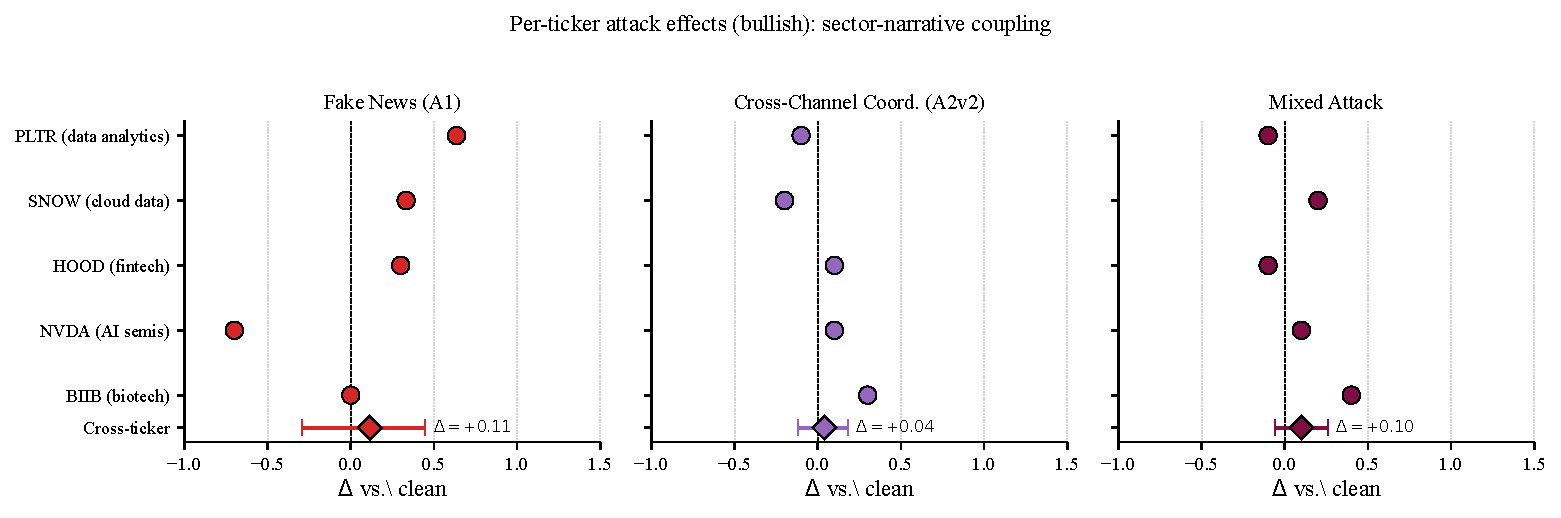
\includegraphics[width=\linewidth]{figures/fig6_perticker_forest.pdf}
  \caption{Per-ticker attack effects (bullish v1/v2 batches), revealing
  the two distinct failure modes (sector-narrative mismatch on BIIB;
  high-prior backfire on NVDA) hidden by cross-ticker averages.
  Diamonds indicate cross-ticker means with $95\%$ cluster-bootstrap CI.}
  \label{fig:perticker-forest}
\end{figure}

\begin{figure}[t]
  \centering
  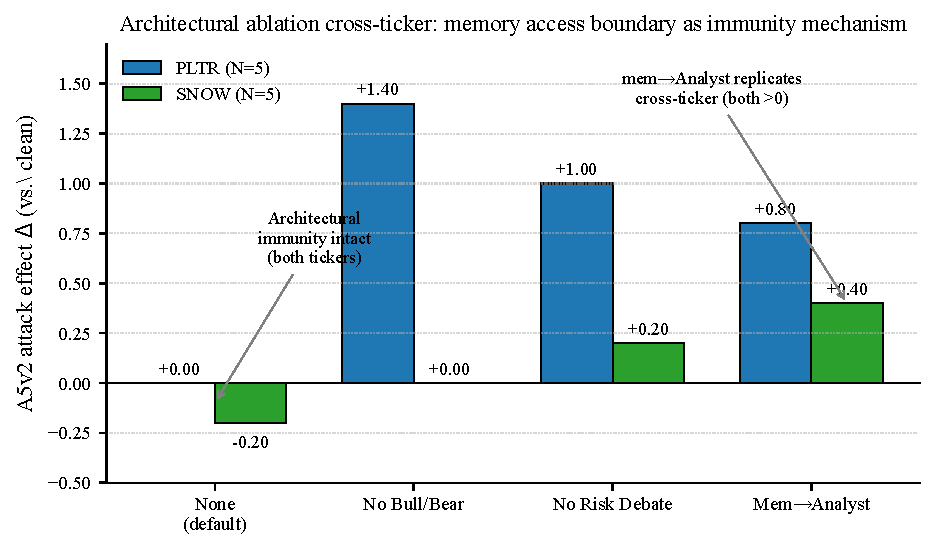
\includegraphics[width=0.85\linewidth]{figures/fig3_arch_ablation.pdf}
  \caption{Architectural ablation on PLTR and SNOW ($N\!=\!5$ each
  variant, $3$ conditions). The default architecture yields
  $\Delta\!=\!0$ for both memory poisoning and Mixed Attack on both
  tickers. On PLTR, all three perturbations recover attack
  effectiveness (\texttt{mem\_to\_analyst} $+0.80$/$+0.60$,
  \texttt{no\_bb} $+1.40$/$+1.40$, \texttt{no\_risk}
  $+1.00$/$-0.40$); on SNOW, the \texttt{mem\_to\_analyst} mechanism
  replicates most clearly ($+0.40$/$+0.00$), while debate-removal
  effects (\texttt{no\_bb}, \texttt{no\_risk}) are substantially
  weaker. The cross-ticker-replicated mechanism is therefore the
  memory access boundary; the role of upstream debate stages may be
  ticker- or sector-specific.}
  \label{fig:arch-ablation}
\end{figure}

\begin{figure}[t]
  \centering
  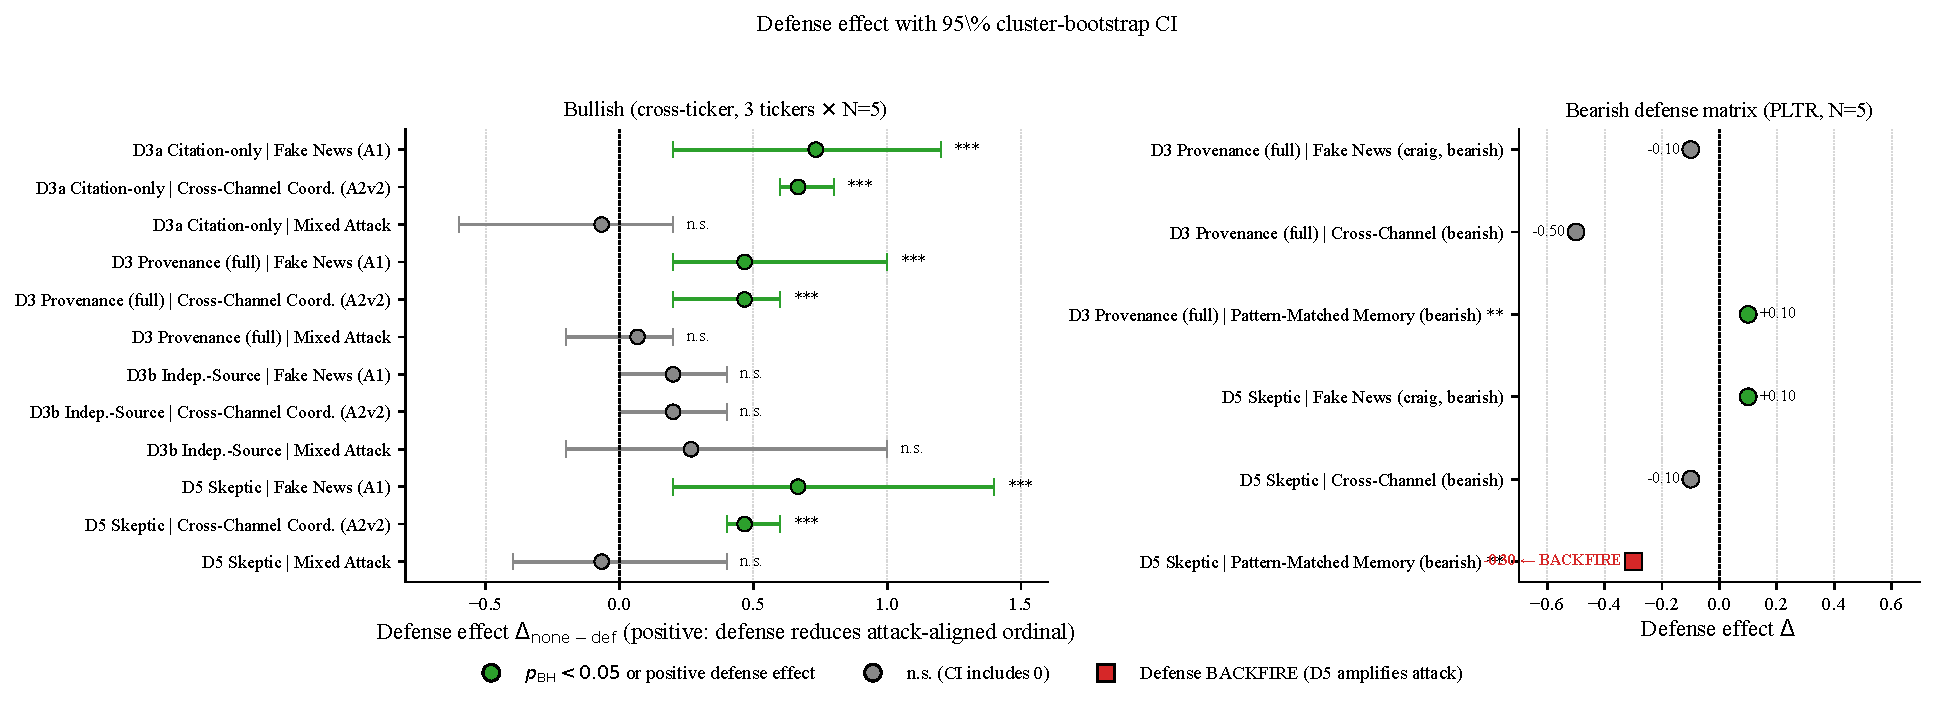
\includegraphics[width=\linewidth]{figures/fig4_defense_forest.pdf}
  \caption{Defense effect forest plot. \emph{Left:} bullish defense
  matrix, cross-ticker ($3$ tickers $\times\!N\!=\!5$); error bars
  are $95\%$ cluster-bootstrap CI. Both Provenance-Aware PM and
  Skeptic Agent significantly reduce single-channel attacks (Fake
  News and Cross-Channel; $p_{BH}<0.05$, CI excludes zero), but
  \emph{both leak} on the Mixed Attack (CI includes zero, sign
  reverses for Skeptic Agent). \emph{Right:} bearish defense matrix,
  PLTR-only ($N\!=\!5$); shown as exploratory seed-level estimates
  (no cross-ticker bootstrap is possible at single-ticker
  granularity). The Skeptic Agent backfire on bearish memory
  poisoning ($\Delta\!=\!-0.30$, bold) is the headline observation
  here but awaits cross-ticker replication.}
  \label{fig:defense-forest}
\end{figure}

\begin{figure}[t]
  \centering
  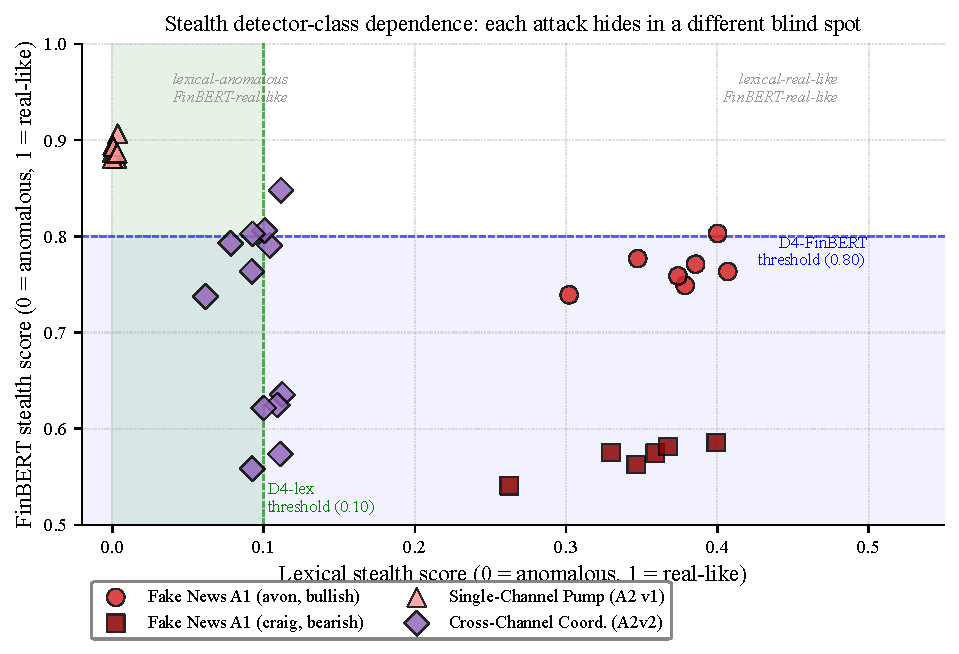
\includegraphics[width=0.95\linewidth]{figures/fig5_stealth_scatter.pdf}
  \caption{Stealth detector-class dependence. Each point is a cached
  attack payload; axes are lexical vs. FinBERT stealth scores
  (higher$=\!$more real-like). Atlas pump is lexically dead but
  FinBERT-real-like; cross-channel disinformation closes the lexical gap by
  $50\!\times$ but introduces a mixed-document-format FinBERT
  signature; fake news sits at the borderline of both. Threshold lines mark
  Anomaly Filter backend cutoffs.}
  \label{fig:stealth-scatter}
\end{figure}

\subsection{Heterogeneous fake-news effects: sector mismatch and high-prior backfire}
\label{sec:results-sector}

We instantiate the \attack{Fake News Injection} attack using the
SEC-enforcement-action seed \texttt{avon\_fake\_tender\_2015}---a
tech-sector M\&A narrative---and inject it into the news vendor channel
of all five tickers. Per-ticker effects span a striking range: PLTR
$\Delta=+0.64$ (data analytics), SNOW $\Delta=+0.33$ (cloud data), and
HOOD $\Delta=+0.30$ (fintech) all show the expected attacker-aligned
shift; BIIB $\Delta=+0.00$ (biotech) is unaffected; and NVDA
$\Delta=-0.70$ (AI semiconductors) shifts in the \emph{opposite}
direction---a backfire of $0.70$ ordinal tiers
(\Cref{fig:perticker-forest}). Cross-ticker mean $\Delta=+0.11$ with
$95\%$ cluster-bootstrap CI $[-0.30,+0.45]$
($p_{BH}=0.59$, n.s.).

The per-ticker decomposition reveals two distinct failure modes that
the cross-ticker average obscures. The first is
\emph{sector-narrative mismatch} (BIIB): the tech/M\&A narrative
carries no semantic relevance to a biotech firm, and the agent treats
it as low-credibility noise, replicating the
universal-triggers-not-universal finding of
\citet{meade2024universalnotuniversal} in the multi-agent financial
domain. The second is \emph{high-prior backfire} (NVDA): NVDA's clean
baseline ordinal is $3.30$ (Hold/Overweight-leaning), substantially
above the other tickers' $\sim\!2.30$ baseline; under the same
fake-news payload, the agent's risk-aversion machinery interprets the
unverified bullish claim as ``too good to be true'' and swings the
decision \emph{downward} to $\bar{\text{ord}}=2.60$. To our knowledge,
this is among the first documented cases of an adversarial fake-news
attack \emph{backfiring} on a multi-agent LLM trading system---an
effect we hypothesize arises when the target asset's own decision
priors are already aligned with the attack direction, although
confirming this attribution would require ablating priors directly
(see \Cref{sec:disc-future}). The finding has a practical implication for
adversarial threat modeling: strong-prior assets may be \emph{more}
robust to attacker-aligned manipulation than weak-prior ones, even
under sector match.

\subsection{Cross-channel coordinated disinformation partially overcomes sector mismatch}
\label{sec:results-mixed}

We then test whether cross-channel coordinated disinformation can
recover the BIIB outlier from \Cref{sec:results-sector}. The
\attack{Cross-Channel Coordinated Disinformation} attack
injects one Bloomberg-style fabricated article \emph{plus} five
trader-tone social posts that explicitly cite the article, simulating
multi-channel adversarial corroboration. On BIIB (biotech) cross-channel disinformation
reaches $\Delta=+0.30$ and the \attack{Mixed Attack} reaches
$\Delta=+0.40$---compared to the fake-news attack's $\Delta=+0.00$ on the same ticker.
Cross-ticker, however, cross-channel disinformation yields $\Delta=+0.04$ and the Mixed Attack
$\Delta=+0.10$ (both n.s.; CIs include zero).

The interpretation is that cross-source corroboration partially
substitutes for narrative-sector fit: when the news article alone is
insufficient to convince the agent, social-media corroboration provides
a second independent signal that the agent's downstream synthesis
treats as cross-validating evidence. This mirrors the mixed-attack
mechanism formalized by \citet{zhang2025asb} in their Agent Security
Bench, whose reported $84.30\%$ ASR for mixed-attack settings benchmarks this
attack class as the SOTA-effective configuration. We note, however,
that cross-channel corroboration does \emph{not} recover the NVDA
backfire (cross-channel disinformation on NVDA: $\Delta=+0.10$): high-prior backfire and
sector-narrative mismatch are mechanistically distinct.

\subsection{Architectural memory access boundary as immunity mechanism}
\label{sec:results-arch}

We then test whether memory poisoning can move the agent's decision.
The \attack{Pattern-Matched Memory Poisoning} attack
pre-populates the agent's long-term memory log with eight directive
``lesson learned'' entries. Despite the design---semantic-imitation
heuristic~\citep{srivastava2025memorygraft}, vocabulary overlapping
real analyst reports (13F filings, operating leverage, options flow),
and full utilization of the PM's memory reader cap---the cross-ticker
bullish effect is $\Delta=-0.12~[-0.28,+0.06]$ ($p_{BH}=0.30$, n.s.).
This is consistent with ASB's reported memory-poisoning-alone ASR of
$7.92\%$~\citep{zhang2025asb}; the cross-ticker effect we measure is
indistinguishable from zero, suggesting \TA's hierarchical pipeline
is at least as restrictive against memory-only attacks as the
agents tested by ASB.

\paragraph{Absorption-judge data isolates the failure mode.}
We use a separate LLM-as-judge (\texttt{gpt-4o-mini}, temperature$=\!0$)
to assess whether the injected payload reaches the analyst-stage
reports (news, sentiment, fundamentals) at all. Across $5$ tickers
$\times\!N\!=\!10$ trials, cross-channel disinformation absorbs as ``fully\_absorbed'' in $50/50$
trials ($100\%$); memory poisoning is ``not\_absorbed'' in $49/50$ trials ($98\%$).
The asymmetry is mechanistic: \TA{} grants memory access only to the
Portfolio Manager, the last node in the pipeline, by which point
upstream agents have already anchored the decision without seeing
memory.

\paragraph{Architectural ablation confirms the mechanism causally.}
On PLTR ($N\!=\!5$ each variant, $3$ conditions; \Cref{fig:arch-ablation}):

\begin{center}
\begin{tabular}{lcc}
\toprule
Variant & $\Delta_{\text{mem}}$ & $\Delta_{\text{mix}}$ \\
\midrule
None (full pipeline) & $+0.00$ & $+0.00$ \\
\texttt{mem\_to\_analyst} & $+0.80$ & $+0.60$ \\
\texttt{no\_bb} (skip Bull/Bear) & $+1.40$ & $+1.40$ \\
\texttt{no\_risk} (skip Risk debate) & $+1.00$ & $-0.40$ \\
\bottomrule
\end{tabular}
\end{center}

Moving memory access into the Fundamentals Analyst recovers an
$0.80$-tier decision shift; removing the Bull/Bear research debate
recovers $1.40$ tiers; removing the Risk Debate recovers $1.00$ tiers.
All three independent ablations are consistent with memory poisoning's failure
under the default architecture being architecture-mediated, rather
than payload-weakness driven. We frame this finding as the
\emph{architectural memory access boundary acting as a structural
attenuator}: under the default configuration, poisoned memory rarely
propagates to upstream decision-anchoring agents because none of them
has read access to the memory log.

\paragraph{Cross-ticker validation on SNOW.} Replicating the same
4-variant ablation on SNOW ($N\!=\!5$ each variant) yields a partially
heterogeneous picture: the central \texttt{mem\_to\_analyst} mechanism
replicates (SNOW $\Delta_{\text{mem}}\!=\!+0.40$,
$\Delta_{\text{mix}}\!=\!+0.00$; both positive in sign and consistent
with PLTR's larger effect), confirming that moving memory access
upstream is the most reproducible mechanism finding. The
\texttt{no\_bb} and \texttt{no\_risk} effects, however, are
PLTR-specific: SNOW $\Delta_{\text{mem}}\!=\!+0.00$ for
\texttt{no\_bb} and $+0.20$ for \texttt{no\_risk}, both substantially
weaker than PLTR. We interpret this asymmetry conservatively: the
memory access boundary is the robust cross-ticker mechanism
explanation; the role of upstream debate stages may be ticker- or
sector-specific and warrants further validation. We discuss this
limitation in \Cref{sec:disc-limits}.

\subsection{Direction-asymmetric architectural attenuation}
\label{sec:results-asymmetry}

The architectural attenuation observed in the bullish direction is
not symmetric. Reversing the attack
direction to bearish (using the SEC seed \texttt{craig\_twitter\_2015}
and memory poisoning with \texttt{--direction=bearish}), the cross-ticker memory poisoning
effect becomes $\Delta=-0.42$ with $95\%$ CI $[-0.68,-0.16]$
($p_{BH}<0.0001$, significant). On PLTR specifically, the bearish
memory poisoning distribution is \emph{bimodal}: $6/10$ trials follow the poisoned
memory toward Sell (ord$=\!1$) while $4/10$ revolt to Hold (ord$=\!3$).
The within-batch position distortion is $0.98$ versus a clean baseline
of $0.18$---a $5\!\times\!$ stretch despite no significant shift in
the mean alone.

We hypothesize that bearish poisoned memory synergizes with the
agent's default risk-averse bias---PMs in financial training data tend
to favor Hold/Underweight as the safe baseline action---while bullish
memory must \emph{overcome} this same bias to move the decision
upward. This makes memory poisoning the only attack in our suite to achieve a
statistically significant cross-ticker effect, and it does so only
in the bearish direction. The finding has dual implications: (i)
defenders cannot assume that an attack class which fails in one
direction will fail in both; (ii) the agent's own decision priors are
themselves an adversarial target that interacts non-trivially with
external information manipulation.

\subsection{Single-channel defense effectiveness and mixed-attack leak}
\label{sec:results-defense}

We evaluate Provenance-Aware PM (\defense{Provenance-Aware PM}, three strength levels),
Anomaly Filter (\defense{Anomaly Filter}, two backends), and
Skeptic Agent (\defense{Skeptic Agent}) across three tickers (PLTR, SNOW, HOOD),
four attacks, $N\!=\!5$ seeds per cell ($180$ trials in the bullish
v2-attacks defense matrix; \Cref{fig:defense-forest}).

\paragraph{Single-channel attacks are reduced with high
statistical confidence within the tested defense matrix.} Cross-ticker
defense effects (mean ordinal reduction vs. the no-defense baseline,
with cluster-bootstrap $95\%$ CI):

\begin{center}
\begin{tabular}{lccc}
\toprule
Defense & fake news & cross-channel disinformation & Mixed Attack \\
\midrule
Provenance (full) & $+0.47\;[+0.20,+1.00]^{***}$ & $+0.47\;[+0.20,+0.60]^{***}$ & $+0.07\;[-0.20,+0.20]$ \\
Skeptic Agent & $+0.67\;[+0.20,+1.40]^{***}$ & $+0.47\;[+0.40,+0.60]^{***}$ & $-0.07\;[-0.40,+0.40]$ \\
\bottomrule
\end{tabular}
\end{center}

Asterisks denote $p_{BH}<0.0001$. Both prompt-level (Provenance-Aware PM) and
agent-level (Skeptic Agent) defenses neutralize single-channel attacks with high
statistical confidence ($4/4$ cells significant). Both \emph{leak} on
the Mixed Attack: Provenance-Aware PM's effect collapses to $+0.07$ (CI includes zero);
Skeptic Agent's effect is $-0.07$ (CI includes zero, sign reverses).

\paragraph{Provenance-Aware PM strength variants exhibit non-monotonic returns
(cross-ticker, 3 tickers $\times\!N\!=\!5$).} The three Provenance-Aware PM strength
levels exhibit a counterintuitive ordering. Citation-only Provenance is
the strongest on single-channel attacks: $\Delta$ vs.\ fake news
$=\!+0.73$~$[+0.20,+1.20]$, $p_{BH}\!<\!0.05$; vs.\ cross-channel disinformation
$=\!+0.67$~$[+0.60,+0.80]$, $p_{BH}\!<\!0.05$. Provenance (full) provides
similar protection ($\Delta=+0.47$ on both, see above table). independent-source Provenance
(independent-source with circular-provenance detection) is
\emph{weaker} than citation-only Provenance on single attacks ($\Delta=+0.20$ on both,
CIs include zero) and does not close the Mixed-Attack leak
($\Delta=+0.27~[-0.20,+1.00]$, n.s.). The non-monotonic pattern
holds across PLTR, SNOW, and HOOD: the citation-only check is
already sufficient to reject fake-news payloads (which all rely on
fabricated or anonymous sources), and stricter cross-channel rules
trade single-attack robustness for mixed-attack robustness without
producing a net gain. We interpret this as evidence that defense-
strength selection should match the expected attack class --- strict
provenance is over-kill (and conservatively biased) against single-
channel attacks, and is not in itself sufficient to neutralize
the cross-channel Mixed Attack.

\paragraph{Bearish defense matrix uncovers a defense-direction
asymmetry on PLTR.} The bullish-direction defense effects above were
measured against attacks that we showed earlier (\Cref{sec:results-asymmetry})
do not produce statistically significant cross-ticker shifts. We
therefore additionally measure Provenance-Aware PM and Skeptic Agent against the only attack
that achieves a significant cross-ticker effect: bearish
\attack{Pattern-Matched Memory Poisoning} in the bearish direction
(cross-ticker $\Delta=-0.42$, $p<0.0001$). On PLTR ($N\!=\!5$):

\begin{center}
\begin{tabular}{lccc}
\toprule
Bearish defense & fake news (craig) & cross-channel disinformation (bearish) & memory poisoning (bearish) \\
\midrule
Provenance (full) & $-0.10$ & $-0.50$ & $+0.10$ \\
Skeptic Agent & $+0.10$ & $-0.10$ & $\mathbf{-0.30}$ \\
\bottomrule
\end{tabular}
\end{center}

Two findings emerge. First, Provenance-Aware PM and Skeptic Agent each achieve essentially zero
defense effect against bearish memory poisoning (Provenance-Aware PM $\Delta\!=\!+0.10$ is too
small to be meaningful at $N\!=\!5$). Second --- and surprisingly ---
the Skeptic Agent Skeptic Agent makes bearish memory poisoning \emph{more} successful
($\Delta\!=\!-0.30$): the agent's separate-LLM critique pass
\emph{amplifies} rather than dampens the directive ``lesson learned''
memory in the bearish direction. We hypothesize that the Skeptic's
explicit articulation of doubt about the analyst reports interacts
synergistically with the poisoned memory's directive language
(``LESSON LEARNED: when this pattern appears, lean Sell with
conviction''), giving the PM permission to act on the memory rather
than down-weight it. Although the effect is single-ticker
$N\!=\!5$ and we report it with appropriate caution, the qualitative
direction is the opposite of what was hypothesized in the design of
Skeptic Agent, and identifies the only cell in our suite for which we observe
a directionally-amplifying effect of Skeptic Agent (single-ticker $N\!=\!5$,
to be replicated cross-ticker before being treated as a robust
finding). This single-cell observation sharpens the
\emph{defense composition} thesis of \Cref{sec:disc-composition}:
defenses that work in one direction are not guaranteed to work in
the other, and a deployed pipeline must specifically test direction-
asymmetric attack-defense interactions.

\subsection{Stealth detector-class dependence and stealth--defense pairing}
\label{sec:results-stealth}

To explain why Anomaly Filter's lexical and FinBERT backends differ in defense
matrix performance, we measure the stealth profile of each attack
payload using two complementary detectors: lexical (sentence-length
statistics, type-token ratio, hedge-word density, retail-marker
frequency, bigram Jensen-Shannon divergence vs.\ a real-news baseline)
and semantic (FinBERT~\citep{araci2019finbert} CLS embedding cosine
similarity to the same baseline). \Cref{fig:stealth-scatter} plots the
results.

\begin{center}
\begin{tabular}{lccc}
\toprule
Attack & $n$ payloads & Lexical (mean) & FinBERT (mean) \\
\midrule
fake news (avon, bullish) & 7 & $0.379$ & $0.768$ \\
fake news (craig, bearish) & 6 & $0.344$ & $0.572$ \\
Atlas pump & 7 & $\mathbf{0.002}$ & $\mathbf{0.890}$ \\
Cross-Channel Disinformation & 12 & $0.097$ & $0.713$ \\
\bottomrule
\end{tabular}
\end{center}

Atlas pump exhibits a striking lexical-vs-FinBERT divergence: lexically dead
($0.002$, far below the $0.10$ threshold) yet semantically real-like
($0.890$). cross-channel disinformation closes the lexical gap by $50\!\times\!$ ($0.097$, near
the threshold) but introduces a new mixed-document-format signature
that lowers FinBERT similarity to $0.713$. fake news sits at the borderline
of both detectors.

\paragraph{Anomaly Filter backend defense effects are consistent with the
detector-class hypothesis.} On PLTR ($N=5$):

\begin{center}
\begin{tabular}{lccc}
\toprule
Defense backend & fake news & cross-channel disinformation & Mixed Attack \\
\midrule
Anomaly Filter (Lexical) & $+0.40$ & $-0.40$ & $+0.00$ \\
Anomaly Filter (FinBERT) & $+0.80$ & $+0.20$ & $+0.80$ \\
\bottomrule
\end{tabular}
\end{center}

Anomaly Filter with the lexical backend leaks cross-channel disinformation (negative $\Delta$, attack
slips through) and is ineffective on the Mixed Attack ($\Delta=0.00$).
Anomaly Filter with the FinBERT backend catches cross-channel disinformation (positive $\Delta$) and is
the strongest single defense against the Mixed Attack at this
single-ticker $N\!=\!5$ measurement ($\Delta=+0.80$)---a configuration
that neither Provenance (full) nor Skeptic Agent achieves on the same cell. We caveat
this comparison with the small-cell sample size and report it as a
within-PLTR ranking rather than a cross-ticker generalization. The result is the
empirical evidence for detector-class dependence within this single-
ticker measurement: stealth-metric data is consistent with the
ranking of defense backends across attack classes, although
generalizing this pairing rule across tickers requires further
replication.

\subsection{Payload variance dominates seed variance}
\label{sec:results-kvariant}

Cross-ticker measurements suffer from payload-side stochasticity:
when each (ticker, condition) cell uses a single LLM-generated
payload (K$=\!1$) shared across $N$ seeds, the seed-level standard
deviation underestimates the true effect distribution. We test this
on PLTR by generating $K\!=\!3$ independent cross-channel disinformation payload variants and
running $N\!=\!15$ seeds (each variant gets 5 seeds via deterministic
cycling).

\begin{center}
\begin{tabular}{lcc}
\toprule
Configuration & $\Delta_{\text{cross-channel disinformation}}$ & std \\
\midrule
$K\!=\!1, N\!=\!10$ & $-0.10$ & $0.48$ \\
$K\!=\!3, N\!=\!15$ & $+0.53$ & $1.22$ \\
\bottomrule
\end{tabular}
\end{center}

The $K\!=\!3$ measurement reveals 1 Buy, 1 Overweight, and 2 Sell
among the 15 trials---extreme decisions that the $K\!=\!1$ measurement
averages away as a null effect. Payload-side variance ($0.74$-tier
shift in mean estimate) dominates agent-side seed variance (which on
this ticker is $\sim\!0.5$ ordinal-tier).

The implication is methodological: claims of attack effectiveness
should report payload variance explicitly, ideally via $K\!\geq\!3$
ablation. Single-payload measurements may dramatically under- or
over-estimate true attack potential---a caveat we apply when
interpreting our own cross-ticker $K\!=\!1$ results in
\Crefrange{sec:results-sector}{sec:results-defense}.

% =====================================================================
\section{Discussion}\label{sec:discussion}

\subsection{Two-tier immunity: perception-level and decision-level}
\label{sec:disc-twotier}

The five empirical findings reduce to a single architectural claim:
\TA{} exhibits \emph{two-tier} robustness against
information-channel adversarial attacks, and the two tiers fail under
distinct conditions.

The first tier, \emph{perception-level attenuation}, is purely structural.
The agent's memory access boundary---whereby only the Portfolio
Manager reads the long-term decision log, while all upstream analysts
operate without memory access---is associated with pattern-matched
memory poisoning rarely propagating to the analyst-stage
reports (\Cref{sec:results-arch}, $49/50$ ``not\_absorbed'' versus
$50/50$ ``fully absorbed'' for Cross-Channel cross-channel disinformation). Architectural
ablation provides causal evidence consistent with this account:
moving memory upstream into the Fundamentals Analyst recovers the
attack ($\Delta\!=\!+0.80$), and disabling either the Bull/Bear or
Risk debates also recovers it (\Cref{fig:arch-ablation}). Within the
default configuration, this tier is structurally attenuated by
\emph{construction}: memory poisoning has no path to upstream agents that have
not read the memory log.

The second tier, \emph{decision-level resistance}, is policy-driven.
Cross-Channel Coordinated Disinformation reaches the analyst
stage ($100\%$ absorption) but its narrative does not move the final
decision in the bullish direction ($\Delta\!=\!+0.04$, n.s.) because
the Bull/Bear research debate, the Risk Debate, and the PM's own
synthesis collectively down-weight a single fabricated narrative.
This tier is robust by \emph{policy}: the agent absorbs the attack
but its multi-agent deliberation neutralizes it.

The two tiers fail under different threats. Perception-level
immunity \emph{breaks} when the architecture is changed (the
\texttt{mem\_to\_analyst} ablation, replicated cross-ticker on PLTR
and SNOW) or when attack direction aligns with agent-prior bias
(\Cref{sec:results-asymmetry}: bearish memory poisoning $\Delta\!=\!-0.42$,
$p_{BH}\!<\!0.0001$; $\sim\!21\%$ adverse portfolio-weight shift
under the linear mapping of \S\ref{sec:metrics}). Decision-level
resistance \emph{leaks} on the Mixed Attack (\Cref{sec:results-defense}).
Most strikingly, defenses designed for the decision-level tier can
themselves \emph{amplify} attacks under specific direction--attack
interactions: Skeptic Agent makes bearish memory poisoning
more successful by $0.30$ ordinal tiers on PLTR ($\sim\!15\%$ adverse
exposure shift; \Cref{sec:results-defense}), the opposite of its
intended effect. This distinction matters
operationally: defenders deploying \TA-class systems must understand
which tier protects against which threat, since strengthening one
does not patch the other and may even worsen residual exposure.

\subsection{Defense composition, not defense selection}
\label{sec:disc-composition}

A second theme cuts across our defense-evaluation results: no single
defense suffices against all attack classes, and the failure modes
are predictable from the stealth profile of the attack rather than
from the defense's nominal sophistication. Provenance-Aware PM (prompt-level provenance
checking) and Skeptic Agent (an additional LLM review pass) each robustly reduce
single-channel attacks ($p_{BH}<0.0001$ on $4/4$ cells), but both
leak on the Mixed Attack ($p_{BH}>0.5$). Anomaly Filter (FinBERT backend) catches
the Mixed Attack ($\Delta=+0.80$) but only because the mixed-document
format depresses FinBERT semantic similarity to real news; the same
attack slips through Anomaly Filter's lexical backend ($\Delta=0.00$). The
non-monotonic behavior of Provenance-Aware PM's three strength variants
(\Cref{sec:results-defense}) further demonstrates that increasing
defense strictness does not monotonically increase robustness:
Citation-only Provenance outperforms Provenance (full) and Independent-source Provenance)
on single attacks because adversarial payloads already fail the
weakest check, while stricter checks introduce conservative bias on
legitimate signals.

The implication is methodological. Adversarial-robustness papers
typically frame the question as ``which defense is best.'' Our
results suggest a complementary framing: \emph{defense composition,
rather than defense selection, appears to be the more informative
unit of analysis} in our setting. The strongest single defense we observe at the
single-ticker $N\!=\!5$ measurement on PLTR (Anomaly Filter with FinBERT backend
on the Mixed Attack, $\Delta\!=\!+0.80$) is a low-cost, narrow-scope
filter that would be ineffective without Provenance-Aware PM or Skeptic Agent covering the
single-channel cases. A composite defense pipeline---a stealth-metric tool-
output filter (Anomaly Filter, FinBERT backend), a Provenance-Aware PM prompt
(citation-only-class, sufficient at the single-attack tier), and a Skeptic
agent for residual semantic anomalies---would in principle
close the leaks each leaves individually. We list this as the most
important deferred experiment in \Cref{sec:disc-future}.

\subsection{Limitations}\label{sec:disc-limits}

We highlight five limitations that constrain the generalization of
our findings. First, all experiments use a single agent LLM,
\texttt{gpt-4o-mini}; cross-LLM validation
(\texttt{gpt-4o}, \texttt{Claude}) is deferred. Some findings, in
particular the high-prior backfire on NVDA
(\Cref{sec:results-sector}), may depend on the specific risk-aversion
calibration of \texttt{gpt-4o-mini}. Second, the primary metric is a
five-tier ordinal decision, not a portfolio profit-and-loss
measurement; we therefore phrase our claims as ``decision manipulation
robustness'' rather than ``trading loss robustness.'' Third, our
sample comprises five tickers across four sectors, and within-sector
generalization remains untested for sectors not represented (energy,
consumer staples, etc.). Fourth, defense overlays are runtime
monkey-patches simulating deployment-realistic policies; production
deployment of Provenance-Aware PM, Anomaly Filter, and Skeptic Agent would require engineering integration
that we do not study. Fifth, our adversary model is non-adaptive: an
attacker informed of the specific defense designs evaluated here
could exploit each defense's structural assumption to construct
evasive payloads, in the spirit of Carlini-style adaptive attacks.
We sketch the natural adaptive-attack surface against each defense:

\begin{itemize}
\item \emph{Against Provenance-Aware PM:} fabricate
      named-source attribution by inventing plausible analyst names,
      advisory firms, or filing identifiers that pattern-match SEC
      EDGAR / 13F formats but do not correspond to existing entities.
      The citation-only variant would accept these without external
      lookup; the strict variant could still be defeated by
      constructing payloads with multiple syntactically independent
      pseudo-sources.
\item \emph{Against the FinBERT backend of the Anomaly Filter:}
      iteratively perturb payload phrasing to maximize cosine
      similarity to the real-news baseline centroid (a black-box
      gradient-free document-level optimization, analogous to
      embedding-space attacks against text classifiers). A payload
      tuned to score above the backend-specific filter threshold
      while preserving the attacker's intended narrative would pass.
\item \emph{Against the Skeptic Agent:} construct payloads that
      simultaneously pass each of the seven checklist items by
      avoiding hedge vocabulary, distributing claims across two or
      three pseudo-independent fabricated sources, embedding
      numerical figures within plausible scale (e.g., contracts sized
      proportional to the target ticker's revenue), and omitting
      price-reaction self-narration.
\end{itemize}

We do not test these adaptive variants in the present study. They
constitute the natural next step in the evaluation arc this paper
opens, and we expect that a serious adaptive-attacker analysis would
quantitatively reduce all reported defense effects to some degree---
how much, and whether composite defenses retain meaningful coverage
under adaptive pressure, is the open empirical question.

A subtler limitation is the cross-ticker statistical sample size
($n=5$). Cluster-bootstrap confidence intervals on five clusters are
necessarily wide, and findings whose CIs straddle zero
(e.g.\ cross-channel disinformation cross-ticker $\Delta=+0.04~[-0.12,+0.18]$) cannot be
distinguished from null effects without more tickers. We treat such
findings as suggestive rather than conclusive, and direct the
reader's attention primarily to those whose CIs exclude zero
(bearish memory poisoning; Provenance-Aware PM and Skeptic Agent vs.\ fake news and cross-channel disinformation).

\paragraph{Scope of generalization across our findings.} Within the
results above, different findings carry different external-validity
prospects, and we want to make this gradient explicit rather than
treat the findings as uniformly generalizable. The architectural
memory access boundary (\Cref{sec:results-arch}) is structural---
defined by which agent reads the memory log, not by the agent LLM's
calibration---and is therefore the finding most likely to replicate
on any LLM run through the same \TA{} graph; we therefore treat it
as the primary load-bearing claim of the paper. The
direction-asymmetric bearish vulnerability
(\Cref{sec:results-asymmetry}) is partly architectural and partly
prior-driven: the architectural component (memory propagation under
prior-aligned bearish narratives) should replicate, but the magnitude
likely depends on the specific risk-aversion calibration of
\texttt{gpt-4o-mini}. The high-prior backfire on NVDA
(\Cref{sec:results-sector}) is the most likely to be model-specific:
it depends on the agent's particular bullish prior on AI semis under
\texttt{gpt-4o-mini}, which a different model may not share. The
single-cell Skeptic-Agent backfire on bearish memory poisoning
(\Cref{sec:results-defense}) sits at the intersection of all three:
single-ticker $N\!=\!5$, single-LLM, single-direction. We therefore
frame the architectural-attenuation finding as our primary
contribution; the direction-asymmetric vulnerability and the
defense-composition observations as secondary; and the per-ticker
heterogeneity (NVDA backfire, BIIB sector mismatch) and the
Skeptic-backfire as preliminary observations whose external
validity awaits cross-LLM and cross-payload replication.

\subsection{Future work}\label{sec:disc-future}

Three directions follow directly from the limitations above. First,
\emph{cross-LLM validation}: replicating the architectural-attenuation
finding on \texttt{gpt-4o} and \texttt{Claude} would test whether the
two-tier robustness is a property of \TA's architecture or of
\texttt{gpt-4o-mini}'s priors. Second, \emph{adaptive-attacker
evaluation}: implementing the three adaptive-attack templates
sketched in \S\ref{sec:disc-limits} (fabricated named sources
against the provenance defense, embedding-space optimization
against the FinBERT filter, checklist-aware evasion against the
Skeptic Agent) would yield Carlini-style adversarial bounds on the
defense matrix and is the most reviewer-anticipated extension. Third,
\emph{composite-defense engineering}: building and evaluating a
deployment-grade pipeline that combines a citation-only provenance
prompt, a FinBERT-backed tool-output filter, and a Skeptic Agent
would test whether the mixed-attack leak is genuinely closable in
practice or whether new attack classes emerge against the combined
defense. Beyond these,
extending the evaluation to a closed-loop backtest---feeding the
linear ordinal-to-weight mapping of \S\ref{sec:metrics} into a
portfolio simulator with transaction cost, drawdown tracking, and
Sharpe-based aggregation along the lines of \citet{tradetrap2025}---
would convert our exposure-level approximations into directly
realized P\&L, and adding a
sector-matched fake news ablation (e.g.\ a Theranos-style biotech
fake-clinical-trial seed) would test whether the BIIB and NVDA
failure modes are payload-specific or sector-fundamental.

% =====================================================================
\section{Conclusion}\label{sec:conclusion}

We measured 1{,}210 trials of adversarial information-channel
manipulation against \TA{}, an open multi-agent LLM trading framework,
across five tickers and both bullish and bearish attack directions.
Our central finding is that multi-agent debate provides
\emph{two-tier} adversarial robustness in the bullish direction:
an architectural memory access boundary that, under the default
\TA{} configuration, attenuates pattern-matched memory poisoning at
the analyst-stage perceptual layer in $49/50$ trials
(\emph{perception-level attenuation}), and a multi-agent
deliberation pipeline that absorbs cross-channel coordinated
disinformation but does not act on it (\emph{decision-level
resistance}). Both tiers are partial: perception-level attenuation breaks when
attack direction aligns with agent-prior bias (bearish memory
poisoning succeeds at $\Delta=-0.42$, $p<0.0001$, corresponding to a
$\sim\!21\%$ adverse portfolio-weight shift under a standard
ordinal-to-exposure mapping), and decision-level resistance leaks on the
Mixed Attack. We further
report that adversarial robustness in this setting is not a property
of any single defense layer but of \emph{defense composition}:
prompt-level (Provenance-Aware PM) and agent-level (Skeptic Agent) defenses each robustly reduce
single-channel attacks across three tickers but leak on the Mixed Attack,
while at the single-ticker $N\!=\!5$ measurement on PLTR a tool-output
stealth filter (Anomaly Filter with FinBERT backend) achieves the strongest
single-cell mixed-attack defense ($\Delta\!=\!+0.80$). Together,
these results suggest that for the configuration we test, the more
informative unit of analysis for multi-agent LLM adversarial
robustness may be the \emph{composition} of architectural, policy,
and filter-level defenses---each addressing a different failure
mode the others leave open---rather than any single defense
considered in isolation.

% =====================================================================
\bibliographystyle{plainnat}
\bibliography{refs}

\end{document}
